\documentclass[border=8pt]{standalone}
\usepackage[T1]{fontenc}
\usepackage{amsmath,amssymb}
\usepackage{mathptmx}
\usepackage{xcolor}
\usepackage{tikz}
\usetikzlibrary{arrows.meta,positioning,fit,calc,backgrounds}
\definecolor{elblue}{HTML}{2A78D6}
\definecolor{foorange}{HTML}{EB6834}
\definecolor{inkgray}{HTML}{52514E}
\begin{document}
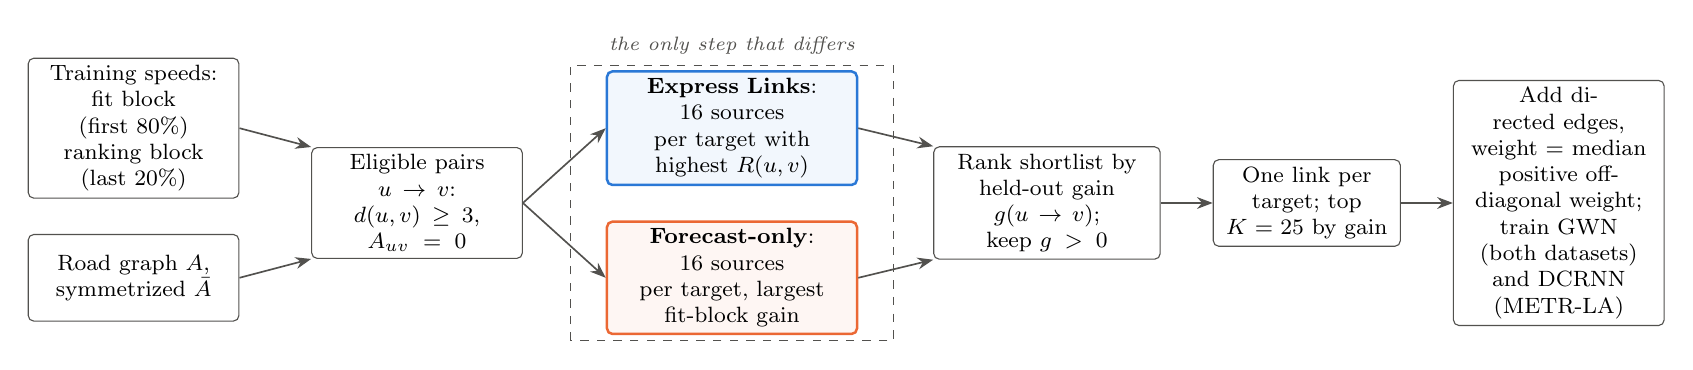
\begin{tikzpicture}[font=\footnotesize,
  box/.style={draw=inkgray, rounded corners=2pt, align=center, minimum height=11mm, inner sep=2.5pt, fill=white},
  el/.style={box, draw=elblue, line width=0.9pt, fill=elblue!6},
  fo/.style={box, draw=foorange, line width=0.9pt, fill=foorange!6},
  arr/.style={-{Stealth[length=2mm]}, inkgray, line width=0.6pt}]
\node[box, text width=25mm] (data) at (0,0.95) {Training speeds:\\fit block (first 80\%)\\ranking block (last 20\%)};
\node[box, text width=25mm] (graph) at (0,-0.95) {Road graph $A$,\\symmetrized $\bar A$};
\node[box, text width=25mm] (elig) at (3.6,0) {Eligible pairs $u\!\to\!v$:\\$d(u,v)\ge 3$, $A_{uv}=0$};
\node[el, text width=30mm] (elsl) at (7.6,0.95) {\textbf{Express Links}: 16 sources\\per target with highest $R(u,v)$};
\node[fo, text width=30mm] (fosl) at (7.6,-0.95) {\textbf{Forecast-only}: 16 sources\\per target, largest fit-block gain};
\node[box, text width=27mm] (rank) at (11.6,0) {Rank shortlist by\\held-out gain $g(u\!\to\!v)$;\\keep $g>0$};
\node[box, text width=22mm] (pick) at (14.9,0) {One link per\\target; top\\$K=25$ by gain};
\node[box, text width=25mm] (train) at (18.1,0) {Add directed edges,\\weight $=$ median\\positive off-diagonal weight;\\{train GWN (both datasets)}\\{and DCRNN (METR-LA)}};
\draw[arr] (data.east) -- (elig.north west);
\draw[arr] (graph.east) -- (elig.south west);
\draw[arr] (elig.east) -- (elsl.west);
\draw[arr] (elig.east) -- (fosl.west);
\draw[arr] (elsl.east) -- (rank.north west);
\draw[arr] (fosl.east) -- (rank.south west);
\draw[arr] (rank) -- (pick); \draw[arr] (pick) -- (train);
\draw[dashed, inkgray] (5.55,-1.75) rectangle (9.65,1.75);
\node[font=\scriptsize\itshape, text=inkgray] at (7.6,2.0) {the only step that differs};
\end{tikzpicture}
\end{document}
